\question{Оптические квантовые генераторы. Лазеры. Условие генерации. 
Пороговый коэффициент усиления.}

Лазерное излучение основано на эффекте усиления спонтанного излучения за 
счет индуцированного внешнего электромагнитного поля, т. е. создания инверсии 
населенностей, при котором происходит вынужденное излучение. Само английское 
слово <<laser>> представляет собой аббревиатуру фразы <<Light Amplification by 
Stimulated Emission of Radiation>>, которая переводится как <<усиление света з
а счет вынужденного испускания излучения>>.

Лазер, оптическая схема которого приведена на рис.\ref{img12.1}, в основном
состоит из трех компонент, а именно: \\
1) активный элемент (АЭ), который усиливает падающую электромагнитную волну; \\
2) система накачки, которая селективно накачивает энергию в активную среду, 
чтобы заселить выбранные энергетические уровни и достичь инверсной 
населенности; \\
3) оптический резонатор, состоящий из двух расположенных друг против друга 
зеркал (М1 и М2) и накапливающий часть индуцированного излучения, 
сконцентрированного в нескольких модах резонатора. 

\begin{figure}[h!]
    \center
    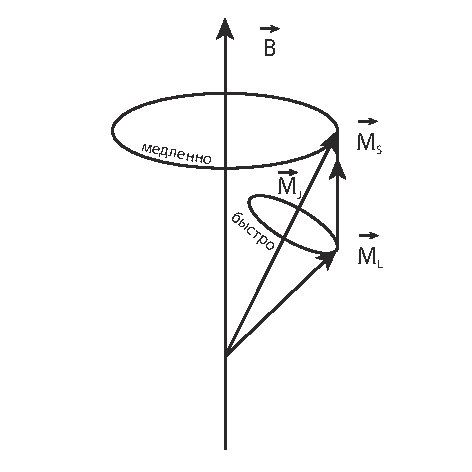
\includegraphics[width=.4\textwidth]{12_01}
    \label{img12.1}
\end{figure}

Усиление электромагнитной волны в среде возможно только при условии, что 
\( N_2 > N_1 \), когда при термодинамическом равновесном состоянии 
\( N_1 > N_2 \). Преобладание индуцированных процессов обусловлено тем, чтобы 
или показатель усиления вещества, через которое проходит свет, был достаточно 
большим, или обеспечивался многократный проход фотонов лазерного излучения 
через усиливающую среду. Среда, в которой осуществлена инверсия населенностей, 
называется активной средой (АС). Увеличение коэффициента усиления АС для 
достижения интенсивного излучения можно достичь увеличением его длины. Однако 
это технически ограничено. Поэтому для получения многократного прохода луча в 
АС ее помещают в резонатор, состоящий из двух параллельных зеркал. Возникшее 
вынужденное излучение после многократного отражения внутри резонатора 
усиливается до такой степени, пока коэффициент усиления \( G \) не 
компенсирует потери излучения, которые обусловлены коэффициентами 
отражения \( R \) и пропускания \( T \) зеркал.

\subquestion{Пороговое условие генерации лазера}
\[ G\cdot R\cdot T > 1 \]
Если зеркала имеют различные коэффициенты отражения \( R_1 \), \( R_2 \) и 
пропускания \( T_1 \), \( T_2 \), то вместо \( R \) и \( T \) используются их 
среднегеометрические значения \( R = \sqrt{R_1 R_2} \), 
\( T = \sqrt{T_1 T_2} \), \( G = \exp[\sigma(N_2 - N_1)d] \)
для критического значения \( (N_2 – N_1)_\text{кр.} \), из порогового условия 
усиления генерации получим:
\[
	(N_2 – N_1)_\text{кр.} \geq \frac{\ln(1/RT)}{\sigma d} \approx
		\frac{1-RT}{\sigma d}
\]
 
Основная проблема создания инверсии населенностей в АЭ состоит в том, что при 
термодинамическом равновесии нижний уровень заселен больше, чем верхние, 
поглощение преобладает над вынужденным излучением. Под воздействием внешнего 
электромагнитного поля совершается больше переходов \( 1 \rightarrow 2 \), чем 
\( 2 \rightarrow 1\). Для энергетической системы из двух уровней действие 
сильного электромагнитного поля приводит только лишь к выравниванию числа 
частиц \( N_1 = N_2 \) между уровнями. Такой эффект называется двухуровневым 
насыщением.

Таким образом, использовав только два уровня, невозможно создать инверсию 
населенностей. Поэтому для создания инверсии населенностей необходимо из 
множества всевозможных энергетических уровней выбрать не менее трех 
энергетических уровней. В зависимости от количества энергетических уровней, 
использованных в принципе действия лазера, они так и называются. 
Например -- трехуровневый, четырехуровневый и т. д. лазеры.
